\documentclass[a4paper,11pt,titlepage]{article}

\newcommand{\MEM}{Moorman}
\newcommand{\KM}{May}
\newcommand{\SK}{Kress}
\newcommand{\MM}{Marin}
\newcommand{\JN}{Nanda}

\usepackage{vhistory}
\usepackage{graphicx}
\usepackage{enumerate}
\usepackage{xspace}
\usepackage{amsmath}
\usepackage{import}
\usepackage{expdlist}


% title definition
\author{Team G2 \\
        Seth Kress\\ 
        Kenny May\\ 
        Michael Moorman\\
        Jagriti Nanda\\
        Misael Marin}
\title{Software Requirements Specification for Dynamic Ad-Hoc Routing Simulator  (SRS v\vhCurrentVersion)}

\date{\today}

\begin{document}

%generate the title page
\maketitle


%generate the table of contents
\tableofcontents

\newpage

\begin{versionhistory}
% Note the syntax of \vhEntry! Authors are separated by `|'         %%
\vhEntry{1.0}{2010-10-03}{\MEM|\KM|\SK|\MM|\JN}{Initial version.}            %%
\end{versionhistory}

\newpage

\section{Introduction}

\subsection{Purpose}

This SRS describes the initial version of the Dynamic Ad-Hoc Routing Simulator (DARS). It
includes specifications for the entire simulator. Particularly, it will provide an overall description
of the functional requirements, necessary features, and required interfaces needed in the
delivered product.

\subsection{Document Conventions}
Requirements or features will be arranged hierarchically where appropriate and sorted
by priority. Detailed requirements will be grouped into more general requirements.
\subsection{Intended Audience and Reading Suggestions}
This document is intended to be read by people involved with the DARS project. This includes
the developers, users, customer, and quality assurance testers. People who are intimately
familiar with the DARS project may choose to skip ahead to section 3 where system features
are described in detail. Those who are new to the DARS project are encouraged to review
section 2 of this document for a review of the current situation relative to Ad-Hoc simulators.

\subsection{Project Scope}
The DARS Simulator is a program written for class CS 524. It is an open source product
designed to help the user to understand how a message is sent to a destination using
the implementation of communication protocols and how they behave in a simulated
Adhoc mobile network. The User should be able to setup a virtual network simulation
by adding ``Nodes'', selecting a protocol and clicking a ``play'' button to display a network
simulation.

\subsection{References}
\begin{itemize}
  \item Software Requirements Specification course handout (Dimitoglou, 2010).
\end{itemize}

\section{Overall Description}
\subsection{Product Perspective}
The DARS system will be joining a collection of other open source routing simulators that are
already free to the public, however the DARS system will include many improvements over
existing simulators that are available, such as a friendlier interface and protocol flexibility. The
DARS system will be a stand alone product that is not part of or shared with any other system.

\begin{figure}[!ht]
        \centering
	\label{DARS Architecture} 
        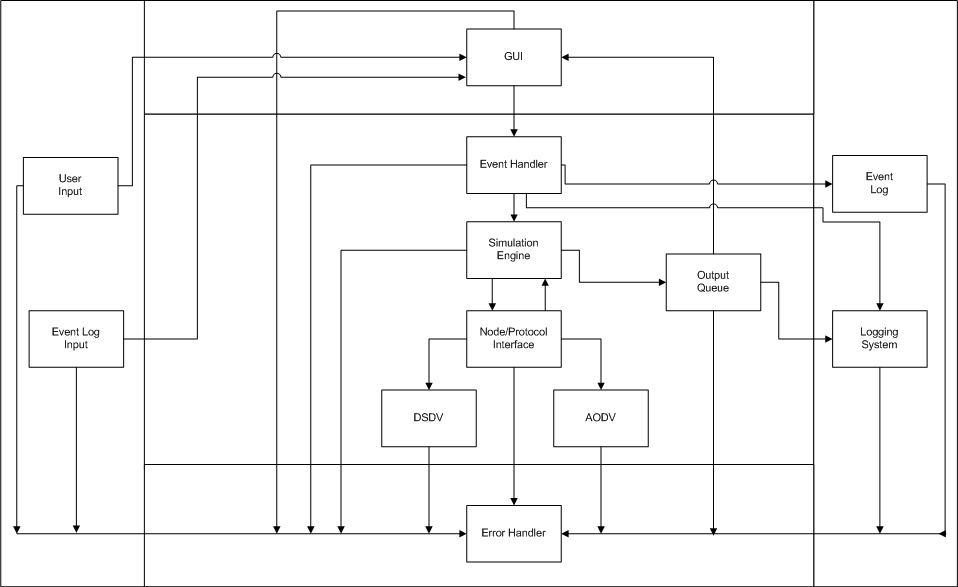
\includegraphics[height=80mm]{img/arch.png}
        \caption{DARS Architecture}
\end{figure}

\subsection{Product Features}
\begin{description}[\breaklabel]
 \item[Adding Nodes] Users will be able to add nodes by right clicking on the simulation area.
 \item[Deleting Nodes] Users will be able to remove nodes by right clicking on a node on the
canvas.
 \item[Editing Node] Users will be able to edit specific attributes of a node by right clicking
on a node on the canvas.
 \item[Moving Nodes] Users will be able to drag a Node around on the canvas to move its
location.
 \item[Interactive Simulation] Once a simulation has started the user will be able to stop,
start, or pause it. Before the simulation has been started the user will be able to
specify the speed that the simulation will execute.
 \item[Dynamic routing] Users will be able which specify which protocol to use during the
simulation via the menu bar when the simulation is first created.
 \item[Replaying Simulation] A user can import a previously run simulation via the menu bar
and re-run it.
 \item[Appealing Graphical Animations] The simulator will be able to show the routing
process to the user with a simple animation that takes place on the node canvas.
 \item[Error Handling] Any errors that occur during a simulation will be displayed to the user
through a status log as well as written to a log file.
 \item[User Help] A help section will be provided to the users to explain the simulator and
assist in starting a simple simulation.
 \item[Platform Independence] The DARS software will be able to run on both Linux and
Windows platforms.

\end{description}

\subsection{User Classes and Characteristics}
There will be three classes of users expected to use the DARS routing simulator, teachers,
students, and editors. Teachers should have more technical expertise than students in that
they should already know how the routing protocols in the simulator function while also having
more time to spend learning the simulator. Their goal will be to demonstrate to students how
the routing protocol works by utilizing animations and logging system. The requirements of the
class should be more heavily based on the clarity of output. Students will be experimenting
on their own to learn how the routing protocols function without much prior experience with
the simulator. The requirements of this class will not only rely on the clarity of the output, but
also the intuitiveness of the GUI to guide them through the simulation construction process.
The student class should be the main focus of our priority because it is the overall goal of this
routing simulator to aid in their education. The last user class is editors. This class should
have sufficient experience operating the simulator but also the desire to expand the software.
The requirements of this last class is more heavily focused on the technical implementation
of the software so that minimal code change will be needed for expansion. The editor class
should be the least important priority of all the classes.

\subsection{Operating Environment}
The DARS software should be operated in a learning environment as well as casual home
user. The targeted hardware platform is a desktop workstation that can either support 32bit
software. The desktop workstation should be running Windows XP, Windows Vista, Windows
7 or any subset of Linux that supports the TAR file format. The targeted platforms are also
expected to have a working version of the java run-time environment installed.
\subsection{Design and Implementation Constraints}
The requirement of software cross-platform compatibility greatly limits the developers options
for design. The amount of languages with a cross platform compatible front end interface is
a very limited number. This was a large factor in the development team’s decision to develop
in a language that was not commonly known amongst the members. Since the software
also needs to be designed in such away that is easily expandable and versatile the planning
process will take an extended amount of time. The simple nature of the software task however
allows the software to run without large hardware requirements.
\subsection{User Documentation}
A help section will be available from the menu bar as well as a read-me file to guide users
through all of the functionality that the DARS software has to offer as well as a troubleshooting
to solve common problems. Programming documentation will be provided for users
that desire to edit or expand the software. This will also be provided as a simple read-me file
that is provided with the software.
\subsection{Assumptions and Dependencies}
Much of this software project is directly dependant of the java development libraries and their
platform compatibility. We are assuming that by using these cross platform libraries that the
functionality will also be the same on all platforms. Any ambiguities in the behavior of the
software between operating systems and functionality could be lost or changed to smooth the
transition.

\section{System Features}
\subsection{Adding Nodes}
\subsubsection{Description and Priority}
Users will be able to add nodes by right clicking on the simulation area canvas.
Having this action available to the user is critical(9) because without this feature the
application is unusable.
\subsubsection{Stimulus/Response Sequences}
A right click on the canvas will reveal a menu that will have the option “add node” that
will place a node at the mouse pointers location with random but valid data.
\subsubsection{Functional Requirements}

\begin{enumerate}[{\bf {REQ} 1}]
  \item This functionality is dependent on the simulators ability to accept new nodes
before, during, and after the routing process has began.
\end{enumerate}

\begin{description}[\breaklabel] 
  \item[Errors] Incorrect buttons pressed during any of the above processes will result in the
   menu closing and the user having to start the process over.
\end{description}

\subsection{Deleting Nodes}

\subsubsection{Description and Priority}
Users will be able to delete nodes by right clicking on the simulation area canvas.
Having this action available to the user is critical(9) because without this feature the
application would not flexible enough to represent a true MANET.

\subsubsection{Stimulus/Response Sequences}
A right click on a node located on the canvas will reveal a menu that will have an
option “delete node” that will remove the node from the canvas.

\subsubsection{Functional Requirements}

\begin{enumerate}[{\bf {REQ} 1}]
  \item This functionality is dependent on the simulators ability to remove nodes
before, during, and after the routing process has began.
\end{enumerate}

\begin{description}[\breaklabel]
  \item[Errors] Incorrect buttons pressed during any of the above processes will result in the
menu closing and the user having to start the process over.
\end{description}

\subsection{Editing Nodes}

\subsubsection{Description and Priority}
Users will be able to edit nodes by right clicking on the simulation area canvas.
Having this action available to the user is critical(9) because without this feature the
application would not flexible enough to represent a true MANET.

\subsubsection{Stimulus/Response Sequences}
A right click on a node located on the canvas will reveal a menu that will have an
option “edit node”. The “edit” menu item will bring a pop-up window to focus filled with
the selected nodes information. This information should now be editable for the user.
From this menu a user may cancel the action or submit the changes.

\subsubsection{Functional Requirements}
\begin{enumerate}[{\bf {REQ} 1}]
  \item Editing a node will be dependant on the routing simulators ability to accept
  new node parameters during the simulator as well as before and after it has
  completed.
\end{enumerate}

\begin{description}[\breaklabel] 
  \item[Errors] Incorrect buttons pressed during any of the above processes will result in the
menu closing and the user having to start the process over.
\end{description}

\subsection{Moving Nodes}
\subsubsection{Description and Priority}
Users will be able to move nodes by drag-and-drop the node in the simulation canvas.
The ability to move a node is needed to produce a realistic simulation of MANETS.
It is critical(9) to provide a way for the user to move a node otherwise the simulator
would not represent a mobile network.
\subsubsection{Stimulus/Response Sequences}
A user can left click and hold on a node and move the cursor to the desired new
location of the node in the simulation canvas and release the left mouse button.
\subsubsection{Functional Requirements}
\begin{enumerate}[{\bf {REQ} 1}]
  \item Moving a node will be dependant on the routing simulators ability to accept a
new node location during the simulator as well as before and after it has completed.\\
\end{enumerate}

\begin{description}[\breaklabel]
  \item[Errors] A user will be presented with an error if they attempt to move a node out of the canvas.
\end{description}

\subsection{Interactive Simulation}
\subsubsection{Description and Priority}
Users will be able to control the pace of the simulation by being able to pause and
resume the simulation as it unfolds. Users will also be able to vary the passage of time
during the simulation. This feature is of high importance (7) because it is necessary to
produce a meaningful simulation. Without this degree of control, the simulation would
be constrained to the arrangement they produced at the beginning of the simulation.
The nature of Ad-Hoc networks is volatile connections and this can only be expressed
within an interactive simulation.
\subsubsection{Stimulus/Response Sequences}
The user will start a simulation after basic simulation parameters are set. After some
amount of time, the user may wish to make a change to the simulation by adding a
network node, deleting a network node, etc. The user will select a pause button in this
case to pause the simulation. After re-working the simulation parameters, the user
would press the resume button. At the end of the user’s simulation they would press
the stop button to end the simulation. The user may augment the passage of within
the simulation at any time by using a slider button. Time may be changed to a value
between 25 percent and 200 percent of default time.
\subsubsection{Functional Requirements}

\begin{enumerate}[{\bf {REQ} 1}]
 \item Simulation must be able pause and resume-able.
 \item Simulation speed must be variable.
\end{enumerate}

\begin{description}[\breaklabel]
  \item[Errors] All errors that occur at this layer of the system likely represent a programming
or logic error. In a bug free system, errors will not be manifested here. If they do occur,
these errors would be outputted to the user through the global error logging interface.
\end{description}

\subsection{Dynamic routing}
\subsubsection{Description and Priority}
Users will be able to select different routing protocols at the initial setup stage of
the simulation. This functionality is moderately(5) important to the overall software
because the simulator will still function with one routing protocol, but it will not be as
useful.
\subsubsection{Stimulus/Response Sequences}
From the simulation menu item located on the menu bar at the top of the program a
drop down will be available with the option “new”. Once the “new” option is highlighted
a sub-menu will be displayed with a list of routing protocols to choose from. After
selecting the desired protocol if any simulation wide parameters need to be specified a
pop-up box will be provided with corresponding entry boxes. These parameters may
include node broadcast intervals or bandwidth levels.
\subsubsection{Functional Requirements}

\begin{enumerate}[{\bf {REQ} 1}]
  \item The drop down menu bar is dependant on java GUI libraries for a functioning
  menu bar.
  \item The option to select multiple routing protocols is directly dependant on the
  completion of both routing protocol options AODV and DSDV.\\
  \item The pop-up window after the protocol selection is dependant on the routing
  protocol requiring simulation wide parameters.
\end{enumerate}
\begin{description}[\breaklabel]
\item[Errors] Incorrect selections or button presses will result in close any menus and
returning users to the main program window.
\end{description}

\subsection{Replaying a Simulation}
\subsubsection{Description and Priority}
The user will be able to save a simulation so that it can be imported into the simulator
at a later time for re-execution and review. During this process however settings may
not be altered because it is a replay not a redo.
\subsubsection{Stimulus/Response Sequences}
During a simulation the most recent status will be displayed in a status bar at the
bottom of the screen. The entire log made up of these statuses will be saved locally
the system. A save simulation button will be placed to the right of the status bar that
will allow the user to save the simulation run to a location to be run at a later date.
This already run simulation can be imported at any time through the “simulation” option
on the menu bar. After this selection is made it will prompt the user for a file location.
This file will then be read in order to set up a new simulation according what was
saved. This replay simulation can be started like a normal simulation.
\subsubsection{Functional Requirements}
\begin{enumerate}[{\bf {REQ} 1}]
  \item Writing and parsing files is dependent on java IO libraries.
  \item Replaying a simulation is dependent on verbose transaction logging.
\end{enumerate}

\begin{description}[\breaklabel]
  \item[Errors]  Errors during file reading or saving will be reported to the user and then they
will be returned back to the main screen for continued use. User miss clicks or wrong
keystrokes will close any menus and return them to the main screen.
\end{description}

\subsection{Appealing Graphical Animations}
\subsubsection{Description and Priority}
Users will be able to view a routing simulation taking place as it happens by viewing a
pictorial animation of the actions taking place. This is a moderately important feature
(6) of the software because visualization is a crucial part of understanding mobile adhoc
networks.
\subsubsection{Stimulus/Response Sequences}
Once the user has setup their simulation and pressed the play button animations will
begin on the canvas indicated the status of messages being sent between nodes in
the simulation. When the user decides to pause of stop the simulation the animation
will also respond accordingly. Upon the selection of a new simulation the canvas will
clear itself. When loading a previous run nodes will be loaded on the canvas as they
were during that particular run.
\subsubsection{Functional Requirements}
\begin{enumerate}[{\bf {REQ} 1}]
  \item Animations are dependent on java GUI libraries.
  \item Animations are dependent on the underlying interface that will give the GUI
  directions.
  \item All above buttons, menus, and drag and drop features will need to be in place
for the entire GUI to work as a whole.
\end{enumerate}

\begin{description}[\breaklabel]
  \item[Errors] Any errors encountered during this process will be reported to the user through
the logging process.
\end{description}[\breaklabel]

\subsection{Verbose Logging}
\subsubsection{Description and Priority}
A significant feature of DARS is the logging of both user input and resultant simulator
output. This feature allows advanced users to parse the results of simulations and
thus produce meaningful statistics. It is of medium importance to deliver this feature
because it does not affect all classes of users.
\subsubsection{Stimulus/Response Sequences}
Every meaningful event that is relevant to the simulation will be recorded into a
tabular log. The log will be actively viewable as the user runs the simulator in a pop
up window. At the end of the simulation the log may be optionally saved to a file in
CSV format, where the user may conduct analysis of the results using the tools of their
choice.
\subsubsection{Functional Requirements}
\begin{enumerate}[{\bf {REQ} 1}]
  \item All simulation relevant events are logged in a human readable and meaningful format.
  \item The log is clearly viewable and active during the simulation.
  \item Logs are savable into a CSV format.
\end{enumerate}

\begin{description}[\breaklabel]
  \item[Errors] The user will be informed of any errors related to the saving of log files.
  They will be given a chance to choose a different destination for the file.
\end{description}

\subsection{Error Handling}
\subsubsection{Description and Priority}
Any errors that may be encountered during the use of the DARS simulator will be
displayed at the bottom of the screen inside of a status bar. This same status will also
be written out to a log file so that it can be viewed later. Depending on the severity
of the error it is also possible that it will throw a warning dialog box up to the user to
alert of them of the problem. This functionality is highly important(8), because without it
there will be nothing to tell the user what has gone wrong.
\subsubsection{Stimulus/Response Sequences}
Errors can be caused by user errors or by the routing protocol malfunctioning.
Depending on which even was the cause of the problem this could generate just a
status log or a both a status log and a screen warning. One example of an error is a
situation where two nodes try to communicate but only the first node has a range long
enough to reach the other. This would result in an error be generated to the status log
along the lines of “Node is out of range to send a message”.
\subsubsection{Functional Requirements}
\begin{enumerate}[{\bf {REQ} 1}]
  \item The status bar must be implemented to display results back to the user.
  \item A file must be writable to keep track of the status log.
\end{enumerate}

\subsection{User Help}
\subsubsection{Description and Priority}
A user help menu will be available to the operator to get them to the point of being able
to set up and run their first simulation. This help section will explain a little bit about
each protocol and give other references that should be used to learn more about the
back-end routing protocols. This is a lower priority(3) because the program can still
function without out this component but it could make it easier to use.
\subsubsection{Stimulus/Response Sequences}
The user will be able to select the help section from a drop down menu on the top of
the screen that will open up a new help document.

\subsubsection{Functional Requirements}
\begin{enumerate}[{\bf {REQ} 1}]
  \item Being able to display a file to the user or possibly html.
\end{enumerate}


\subsection{Platform Independent}
\subsubsection{Description and Priority}
The DARS simulator will be supported on the Windows and Linux operating systems.
This will include installation packages for each OS. This feature is important9) {to enable the
widest possible number of users to DARS.
\subsubsection{Stimulus/Response Sequences}
The user will be able to choose between installing on Windows or Linux.

\subsubsection{Functional Requirements}

\begin{enumerate}[{\bf {REQ} 1}]
  \item  Installing on Windows will require using a native installer, at this point this
technology is TBD.
  \item Each various Linux Distribution uses different package managers. A package
manager(s) will need to be chosen.
\end{enumerate}

\begin{description}[\breaklabel]
  \item[Errors] Errors during the install of DARS will be handled by the respective OS.
\end{description}


\section{External Interface Requirements}
The DARS Simulator is a standalone application and does not require an external interface.
\subsection{User Interfaces}
The primary user interface for the DARS is the Graphical User Interface(GUI). All features
and functionality is accessible via the GUI which will be created using the JAVA SWING
libraries. The GUI for DARS will depend on the standard component set of the SWING
library. In addition to the GUI, DARS will provide the user with log files that can be reviewed
using a standard text editor. The full layout of the GUI will be determined at a later point.
In general, the user interface will follow the user interface design principles outlined by Mandel
in The Golden Rules of User Interface Design (Mandel, 1997). These principles are as
follows:

\begin{enumerate}[1.]
  \item Place users in control.
  \item Reduce user’s memory load.
  \item Make the interface consistent.
\end{enumerate}

The User Interface is implemented via various Java components. The user will be able to right
click on the screen and add, edit and delete Nodes. Also, the user can easily start/Stop the
simulation by clicking on the Play or Pause button.
\subsection{Hardware Interfaces}
The application will interface with display devices, the keyboard, and the mouse through the
Java Runtime Environment.
\subsection{Software Interfaces}
The application will interface with Java’s core libraries throught the Java Runtime
Environment. DARS will have the ability to write log files so it interacts with standard text
editors.
\subsection{Communications Interfaces}
DARS operates in a local environment and does not require any external communication
interface.

\section{Other Nonfunctional Requirements}
\subsection{Performance Requirements}
The DARS will run without a negative impact to the users experience commensurate with the
hardware requirements to support the operating system. Specific hardware requirements if
any will be determined during testing.
\subsection{Safety Requirements}
The DARS will not comply with any safety requirements. The use of this simulator will not
cause any loss or damage to the user’s operating system and hardware.
\subsection{Security Requirements}
This product will be open to the class students, team of students developing it as well as to
the professor. There is no security or privacy issue even if the product is open to the public
because it is meant for educational purposes.
DARS is a standalone program that will not utilize the network or privileged OS functionality
thus limiting its impact on the overall security of the host platform.
\subsection{Software Quality Attributes}
The simulator has some embedded quality characteristics built in it which facilitates customers
and developers to improve usability of product with time. The software is developed in a
way that it can adapts to new requirements very easily. For instance, if a user wants to
operate simulator with routing method other than AODV or DSDV then components for new
protocols can be simply added into the software product. With ever changing requirements of
customers, DARS is flexible, interoperable and portable. It is highly reliable in operation and
its components can be reused for similar projects. DARS is extremely robust in functionality
under any circumstance, it guarantees to give some output after a simulation run otherwise
result an error message to the user. It will be tested for all test cases until found correct under
all situations.
The source code of the product is going to be open as this is going to be open source
software. It will be free for further modifications and improvements.
\section{Other Requirements}
DARS will be released under the GNU GPLv3 license. Additional requirements are TBD.\\

\newpage
\appendix
\section{Definitions}
GUI - Graphical User Interface\\
AODV - Ad-Hoc On Demand Distance Vector\\
DSDV - Destination-Sequenced Distance-Vector Routing\\
DARS - Dynamic Ad-Hoc Routing Simulator\\
MANET - Mobile Ad-Hoc Network
\end{document}
